

%----------------------------------------------------------------------------------------
%	PACKAGES AND OTHER DOCUMENT CONFIGURATIONS
%----------------------------------------------------------------------------------------

\documentclass{article}

\usepackage{fancyhdr} % Required for custom headers
\usepackage{lastpage} % Required to determine the last page for the footer
\usepackage{extramarks} % Required for headers and footers
\usepackage[usenames,dvipsnames]{color} % Required for custom colors
\usepackage{graphicx} % Required to insert images
\usepackage{listings} % Required for insertion of code
\usepackage{courier} % Required for the courier font


% Margins
\topmargin=-0.45in
\evensidemargin=0in
\oddsidemargin=0in
\textwidth=6.5in
\textheight=9.0in
\headsep=0.25in

\linespread{1.1} % Line spacing

% Set up the header and footer
\pagestyle{fancy}
\lhead{\hmwkAuthorName\ : \hmwkStudentID} % Top left header
\chead{ \hmwkClassShort} % Top center head
\rhead{\firstxmark} % Top right header
\lfoot{\lastxmark} % Bottom left footer
\cfoot{} % Bottom center footer
\rfoot{Page\ \thepage\ of\ \protect\pageref{LastPage}} % Bottom right footer
\renewcommand\headrulewidth{0.4pt} % Size of the header rule
\renewcommand\footrulewidth{0.4pt} % Size of the footer rule

\setlength\parindent{0pt} % Removes all indentation from paragraphs

%----------------------------------------------------------------------------------------
%	CODE INCLUSION CONFIGURATION
%----------------------------------------------------------------------------------------

\definecolor{MyDarkGreen}{rgb}{0.0,0.4,0.0} % This is the color used for comments
\lstloadlanguages{C} % Load Perl syntax for listings, for a list of other languages supported see: ftp://ftp.tex.ac.uk/tex-archive/macros/latex/contrib/listings/listings.pdf
\lstset{language=C, % Use c in this example
        frame=single, % Single frame around code
        basicstyle=\small\ttfamily, % Use small true type font
        keywordstyle=[1]\color{Blue}\bf, % cfunctions bold and blue
        keywordstyle=[2]\color{Purple}, % c function arguments purple
        keywordstyle=[3]\color{Blue}\underbar, % Custom functions underlined and blue
        identifierstyle=, % Nothing special about identifiers                                         
        commentstyle=\usefont{T1}{pcr}{m}{sl}\color{MyDarkGreen}\small, % Comments small dark green courier font
        stringstyle=\color{Purple}, % Strings are purple
        showstringspaces=false, % Don't put marks in string spaces
        tabsize=5, % 5 spaces per tab
        %
        % Put standard c functions not included in the default language here
        morekeywords={rand},
        %
        % Put c function parameters here
        morekeywords=[2]{on, off, interp},
        %
        % Put user defined functions here
        morekeywords=[3]{test},
       	%
        morecomment=[l][\color{Blue}]{...}, % Line continuation (...) like blue comment
        numbers=left, % Line numbers on left
        firstnumber=1, % Line numbers start with line 1
        numberstyle=\tiny\color{Blue}, % Line numbers are blue and small
        stepnumber=5 % Line numbers go in steps of 5
}

% Creates a new command to include a script, the first parameter is the filename of the script (without .txt), the second parameter is the caption
\newcommand{\Cscript}[2]{
\begin{itemize}
\item[]\lstinputlisting[caption=#2,label=#1]{#1.txt}
\end{itemize}
}

%----------------------------------------------------------------------------------------
%	DOCUMENT STRUCTURE COMMANDS
%	Skip this unless you know what you're doing
%----------------------------------------------------------------------------------------

% Header and footer for when a page split occurs within a problem environment
\newcommand{\enterProblemHeader}[1]{
\nobreak\extramarks{#1}{#1 continued on next page\ldots}\nobreak
\nobreak\extramarks{#1 }{#1 continued on next page\ldots}\nobreak
}

% Header and footer for when a page split occurs between problem environments
\newcommand{\exitProblemHeader}[1]{
\nobreak\extramarks{#1}{#1 continued on next page\ldots}\nobreak
\nobreak\extramarks{#1}{}\nobreak
}

\setcounter{secnumdepth}{0} % Removes default section numbers
\newcounter{homeworkProblemCounter} % Creates a counter to keep track of the number of problems

\newcommand{\homeworkProblemName}{}
\newenvironment{homeworkProblem}[1][Problem \arabic{homeworkProblemCounter}]{ % Makes a new environment called homeworkProblem which takes 1 argument (custom name) but the default is "Problem #"
\stepcounter{homeworkProblemCounter} % Increase counter for number of problems
\renewcommand{\homeworkProblemName}{#1} % Assign \homeworkProblemName the name of the problem
\section{\homeworkProblemName} % Make a section in the document with the custom problem count
\enterProblemHeader{\homeworkProblemName} % Header and footer within the environment
}{
\exitProblemHeader{\homeworkProblemName} % Header and footer after the environment
}

\newcommand{\problemAnswer}[1]{ % Defines the problem answer command with the content as the only argument
\noindent\framebox[\columnwidth][c]{\begin{minipage}{0.98\columnwidth}#1\end{minipage}} % Makes the box around the problem answer and puts the content inside
}

\newcommand{\homeworkSectionName}{}
\newenvironment{homeworkSection}[1]{ % New environment for sections within homework problems, takes 1 argument - the name of the section
\renewcommand{\homeworkSectionName}{#1} % Assign \homeworkSectionName to the name of the section from the environment argument
\subsection{\homeworkSectionName} % Make a subsection with the custom name of the subsection
\enterProblemHeader{\homeworkProblemName} % Header and footer within the environment
}{
\enterProblemHeader{\homeworkProblemName} % Header and footer after the environment
}

%----------------------------------------------------------------------------------------
%	NAME AND CLASS SECTION
%----------------------------------------------------------------------------------------

\newcommand{\hmwkTitle}{207SE Operating Systems, Security and Networks Portfolio} % Assignment title
\newcommand{\hmwkDueDate}{Monday,\ December\ 15th,\ 2014} % Due date
\newcommand{\hmwkClass}{ECU178 \- Computer Science} % Course/class
\newcommand{\hmwkClassTime}{10:30am} % Class/lecture time
\newcommand{\hmwkClassInstructor}{Dr Mark Elshaw} % Teacher/lecturer
\newcommand{\hmwkAuthorName}{Robert Rigler} % Your name
\newcommand{\hmwkStudentID}{4939377}% My Student ID
\newcommand{\hmwkClassShort}{207SE Portfolio} %Short name for class (only used in header)

%----------------------------------------------------------------------------------------
%	TITLE PAGE
%----------------------------------------------------------------------------------------

\title{
\vspace{2in}
\textmd{\textbf{\hmwkClass:\ \\ \hmwkTitle}}\\
\normalsize\vspace{0.1in}\small{Due\ on\ \hmwkDueDate}\\
\vspace{0.1in}\large{\textit{\hmwkClassInstructor\ }}
\vspace{3in}
}

\author{\textbf{\hmwkAuthorName\ : \hmwkStudentID}}
\date{} % Insert date here if you want it to appear below your name

%----------------------------------------------------------------------------------------

\begin{document}

\maketitle

%----------------------------------------------------------------------------------------
%	TABLE OF CONTENTS
%----------------------------------------------------------------------------------------

%\setcounter{tocdepth}{1} % Uncomment this line if you don't want subsections listed in the ToC

\newpage
\tableofcontents
\newpage

%----------------------------------------------------------------------------------------
%	PROBLEM 1
%----------------------------------------------------------------------------------------

% To have just one problem per page, simply put a \clearpage after each problem

\begin{homeworkProblem}[Item 1 - Linux Command Line]{}
\homeworkSection{1. Logfile containing evidence of activities}
\problemAnswer{

%\Cscript{Assignment_1/ass3}{Log file}
}



\end{homeworkProblem}
\clearpage

%----------------------------------------------------------------------------------------
%	PROBLEM 2
%----------------------------------------------------------------------------------------

\begin{homeworkProblem}[Item 2 - Assembly Code]
\begin{homeworkSection}{1. Right-Angled triangle}
Using x86 Assembly code, draw a Right-angled triangle
\Cscript{Assignment_2/t1/rat}{Right angled triangle}
\problemAnswer{

\begin{center}
Evidence of Right angled triangle
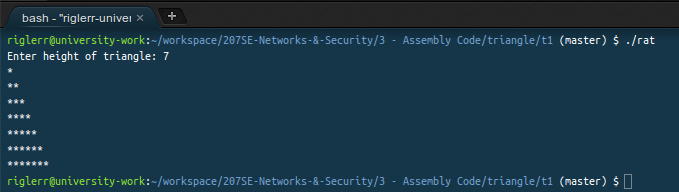
\includegraphics[width=0.9\columnwidth]{Assignment_2/t1/Evi1.png} 
\end{center}

}
\clearpage
\end{homeworkSection}
\begin{homeworkSection}{2. Isosceles Triangle}
Using x86 Assembly code, draw an Isosceles triangle
\Cscript{Assignment_2/t2/iso}{Isosceles Triangle}
\problemAnswer{

\begin{center}
Evidence of triangle
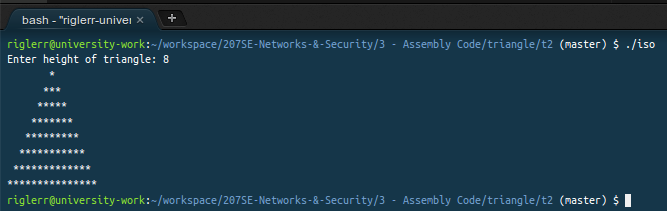
\includegraphics[width=0.9\columnwidth]{Assignment_2/t2/Evi1.png} 
\end{center}

}


\end{homeworkSection}

\end{homeworkProblem}
\clearpage
%----------------------------------------------------------------------------------------
%	PROBLEM 3
%----------------------------------------------------------------------------------------
\begin{homeworkProblem}[Item 3 - Bootloader]{}





\end{homeworkProblem}
\clearpage
%----------------------------------------------------------------------------------------
%	PROBLEM 4
%----------------------------------------------------------------------------------------
\begin{homeworkProblem}[Item 4 - Inside Proc]{}

\homeworkSection{1. List the CPU Information using the Cat Command}
\problemAnswer{
\begin{center}
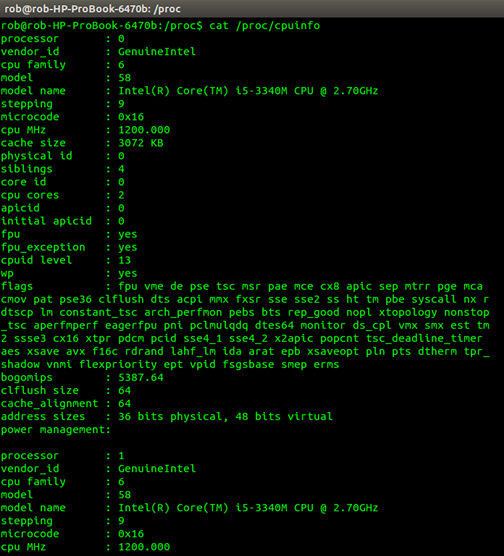
\includegraphics[width=0.75\columnwidth]{Assignment_4/1Cat.png} 
\end{center}
}

\homeworkSection{2.  Show a table of the interrupts on the system}
\problemAnswer{
\begin{center}
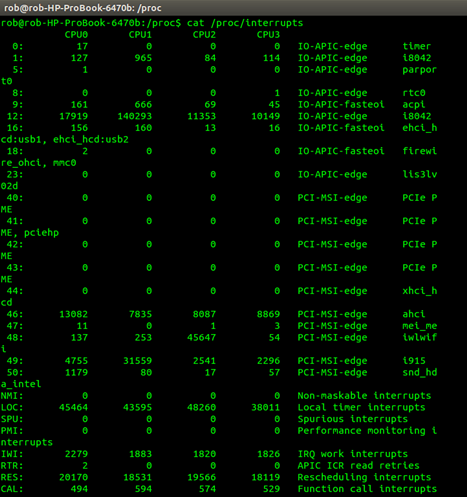
\includegraphics[width=0.75\columnwidth]{Assignment_4/2Table.png}
\end{center}
}

\homeworkSection{3.  Show number of CPUs, the producer of the CPUs and the CPU Model.}
\problemAnswer{
\begin{center}
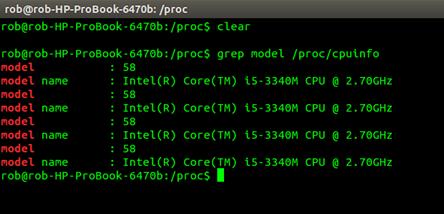
\includegraphics[width=0.75\columnwidth]{Assignment_4/3CPU.png}
\end{center}
}

\homeworkSection{4.  How the parameters that are passed to the kernel when starting up linux.}
\problemAnswer{
\begin{center}
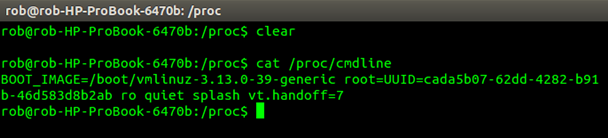
\includegraphics[width=0.75\columnwidth]{Assignment_4/4Paramaters.png}
\end{center}
}

\homeworkSection{5.  Show the name of the output devices and the number of megabytes read per second during the second sampled interval.}
\problemAnswer{
\begin{center}
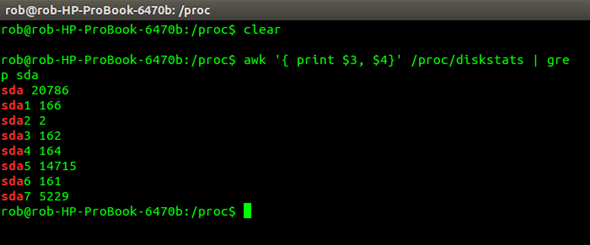
\includegraphics[width=0.75\columnwidth]{Assignment_4/5Disk.png}
\end{center}
}
\clearpage

\homeworkSection{6.  Menu based shell script.}

\Cscript{Assignment_4/BashScript}{Bash Script}




\end{homeworkProblem}
\clearpage
%----------------------------------------------------------------------------------------
%	PROBLEM 5
%----------------------------------------------------------------------------------------
\begin{homeworkProblem}[Item 5 - Buffer tutorial]{}
\homeworkSection{1. Commented version of the rovided code}
\Cscript{Assignment_5/item1}{Commented Buffer Code}
\homeworkSection{2. Evidence of compiled code}

\problemAnswer{ 
\begin{center}
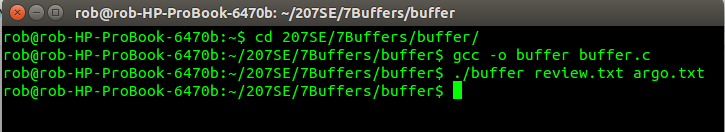
\includegraphics[width=0.75\columnwidth]{Assignment_5/2Compiled.png}\\
 Argo.txt contains the exact same text that was in review.txt
\end{center}
}
\clearpage
\homeworkSection{3. Code adaptation to show how many cahracters were read in total and how many times the buffer was filled}
\Cscript{Assignment_5/item3}{Adpated Code}
\homeworkSection{3a Evidence}
\problemAnswer{
\begin{center}
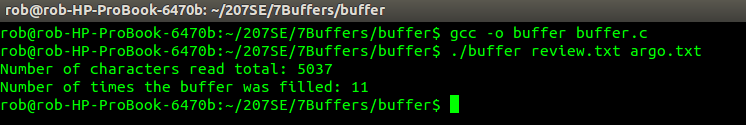
\includegraphics[width=0.75\columnwidth]{Assignment_5/3Evidence.png}
\end{center}}
\homeworkSection{4. Altering the buffer size}
\problemAnswer{
\begin{itemize}
\item Doubling the buffer size to 1000, the program filled the buffer 6 times. This is half of the original value + 1.
\item Doubling the buffer size again to 2000 , the program filled the buffer 3 times which is half of 6.
\item Raising the the buffer size to 10000, the program filled the buffer 1 time, indicating that the entire text was placed into the buffer.
\end{itemize}
There is a direct linear correlation between the buffer size and the amount of times that the buffer was filled.

}
\clearpage

\homeworkSection{5. Adapt the code so that it is possible to compare if two files are the same.}
\Cscript{Assignment_5/item5}{Adapted code}
\homeworkSection{5a. Evidence of comparison between review.txt and argo.txt}
\problemAnswer{
\begin{center}
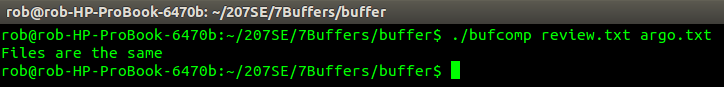
\includegraphics[width=0.75\columnwidth]{Assignment_5/5Comp1.png}
\end{center}
}
\homeworkSection{5b. Evidence of comaprison between argo.txt and reviewobserver.txt}
\problemAnswer{
\begin{center}
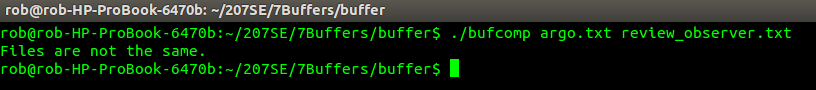
\includegraphics[width=0.75\columnwidth]{Assignment_5/5Comp2.png}
\end{center}
}


\end{homeworkProblem}
\clearpage
%----------------------------------------------------------------------------------------
%	PROBLEM 6
%----------------------------------------------------------------------------------------
\begin{homeworkProblem}[Item 6 - Cache tutorial]{}
\homeworkSection{1. Complete the cr\textunderscore read\textunderscore byte function}
Please see the provided code in cache\textunderscore reader.c 

\homeworkSection{2. Prove the file is being buffered}
To prove the code is being buffered. I included \emph{printf(" \textbackslash n");} on line 58 in the cache\textunderscore reader.c file . The program now starts a new line every time it reaches the end of the buffer ( in this example 20). 

\homeworkSection{3. Provide some statistics}
To count the number of bytes read, I created a variable called \emph{byte\textunderscore tot} in the \emph{cr\textunderscore file}  structure (line12) in the cache\textunderscore reader.h file. This variable is used in the \emph{Refill()} method (line 15). Every time the \emph{Refill()} method is called, it adds the value of \emph{len} (which contains the number of bytes currently being read) to itself.\\
The amount of times the buffer was refilled, was calculated by dividing the number of bytes read from the text by the size of the buffer.




\Cscript{Assignment_6/cache_example}{cache\textunderscore example.c}
\clearpage

\Cscript{Assignment_6/cache_readerh}{cache\textunderscore reader.h}
\clearpage

\Cscript{Assignment_6/cache_reader}{cache\textunderscore reader.c}

%

\end{homeworkProblem}
\clearpage
%----------------------------------------------------------------------------------------
%	PROBLEM 7
%----------------------------------------------------------------------------------------
\begin{homeworkProblem}[Item 7 - Kernell]{}





\end{homeworkProblem}



\end{document}